
%%%%%%%%%%%%%%%%%%%%%%%%%%%%%%%%%%%%%%%%%%%%%%%%%%%%%%%%%%%%%%%%%%%%%%%%%
%           Capítulo 3: Metodologia                   %
%%%%%%%%%%%%%%%%%%%%%%%%%%%%%%%%%%%%%%%%%%%%%%%%%%%%%%%%%%%%%%%%%%%%%%%%%



\chapter{Metodología}
En este capítulo se expone todo el desarrollo de la fuente de alto voltaje en cuestión; diseño del sistema, fabricación del sistema, diseño del firmware del micro controlador, implementación y por último el método experimental.\\

El sistema esta compuesto por dos partes, hardware y firmware, el hardware se compone de tres partes como vemos en la figura 3.5: parte digital de control, inversor de voltaje y rectificador multiplicador. \\

Por otro lado el firmware consiste en los programas que realizan el control completo de la generación de alto voltaje por medio del desarrollo de un ambiente gráfico al que el usuario tiene acceso,  control para la medición de voltajes, corrientes y protecciones necesarias para el correcto funcionamiento del sistema en general, así como también un control para el inversor de voltaje, mediante la implementación de un ADC ( Analog to Digital Converter) a la salida de una devanado de baja en el transformador de alto voltaje el cual controla la salida de alto voltaje.
\newpage


 % The \cite command functions as follows:
 %   \citet{key} ==>>                Jones et al. (1990)
 %   \citet*{key} ==>>               Jones, Baker, and Smith (1990)
 %   \citep{key} ==>>                (Jones et al., 1990)
 %   \citep*{key} ==>>               (Jones, Baker, and Smith, 1990)
 %   \citep[chap. 2]{key} ==>>       (Jones et al., 1990, chap. 2)
 %   \citep[e.g.][]{key} ==>>        (e.g. Jones et al., 1990)
 %   \citep[e.g.][p. 32]{key} ==>>   (e.g. Jones et al., p. 32)
 %   \citeauthor{key} ==>>           Jones et al.
 %   \citeauthor*{key} ==>>          Jones, Baker, and Smith
 %   \citeyear{key} ==>>             1990



\section{Materiales utilizados}

La medición y comprobación del alto voltaje no es tan sencilla si no se tienen las herramientas necesarias para ello. La utilización de osciloscopios (figura 3.3), voltimetros (figura 3.2) y sistemas de medición se ve afectado debido a que en su mayoría los voltajes soportados por los equipos son apenas de unos cuantos miles de volts. Es por ello que en este proyecto se han requerido herramientas como lo son las sondas divisoras de voltaje, similar a la que se aprecia en la figura 3.1, permitiendo así la utilización de las herramientas antes comentadas aquí.\\

\begin{figure}[H]
\centering
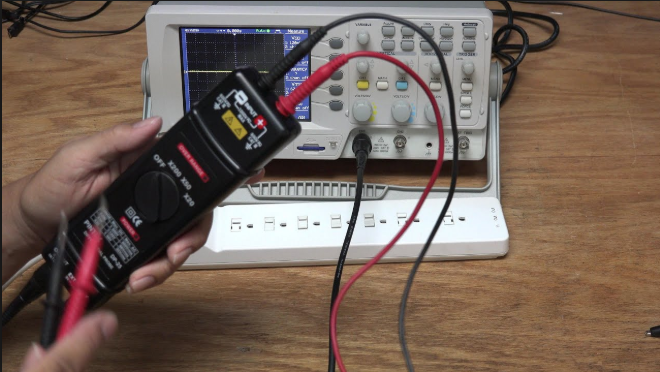
\includegraphics[width=9cm]{Capitulo3/figs/sonda.png}
\caption{Sonda de alto voltaje}
\end{figure}

Con esta herramienta se ha logrado utilizar el osciloscopio con una resolución de 8 bits, de la marca TELEDYNE modelo WavePro y analizar la señal para presentar resultados mas claros. Podemos observar el osciloscopio utilizado para las mediciones y un multimetro de la marca fluke, los cuales son suficientes para determinar la eficiencia de nuestra fuente de voltaje. Teniendo en cuenta siempre la seguridad requerida para la operación de estos instrumentos.


\begin{figure}[H]
\centering
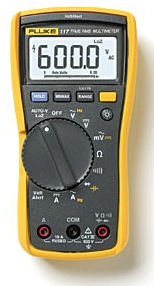
\includegraphics[width=4cm]{Capitulo3/figs/multim.png}
\caption{Multimetro Fluke 116 0.001V de resolución.}
\end{figure}

\begin{figure}[H]
\centering
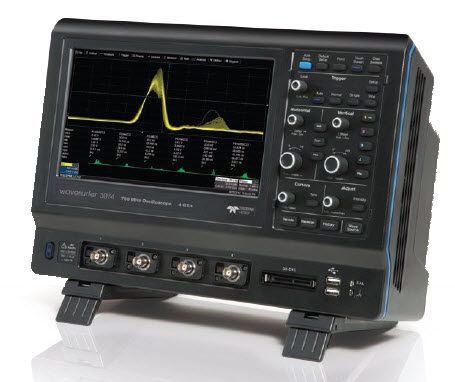
\includegraphics[width=9cm]{Capitulo3/figs/oscilo.png}
\caption{Osciloscopio teledyne lecroy 8 bits de resolución.}
\end{figure}

Para la fabricación de los PCB se utilizó una herramienta LPKF, router computarizado. El cual, una vez hecho el diseño en el programa EAGLE se prosiguió a la generación de los archivos gerber para su posterior maquinación. 

\begin{figure}[H]
\centering
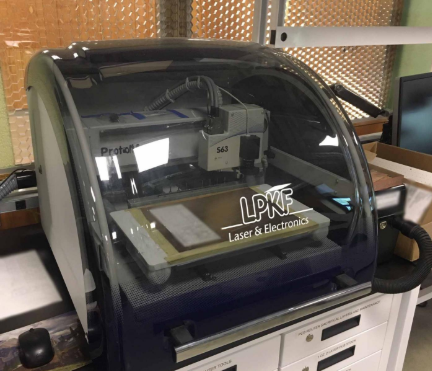
\includegraphics[width=9cm]{Capitulo3/figs/proto.png}
\caption{Router CNC LPKF para maquinado de PCBs.}
\end{figure}
\newpage


%%%%%%%%%%%%%%%%%%%%%%%%%%%%%%%%%%%%%%%%%%%%%%%%%%%%%%%%%%%%%%%%%%%%%%%%%
%                          Descripción de la planta                     %
%%%%%%%%%%%%%%%%%%%%%%%%%%%%%%%%%%%%%%%%%%%%%%%%%%%%%%%%%%%%%%%%%%%%%%%%%
\section{Diseño del hardware}


La figura 3.1 muestra un diagrama a bloques de la estructura general del hardware que conforma el sistema de generación de alto voltaje, el cual esta compuesto, desde la parte superior a la inferior, primeramente por bloques relacionados con el control digital del sistema, este bloque se encarga de las interfaces para el usuario así como también del control e instrumentación de los diferentes sensores, el siguiente conjunto de bloques representan la electrónica encargada de la inversión de voltaje y por ultimo tenemos la rectificación.  \\

\begin{figure}[H]
\centering
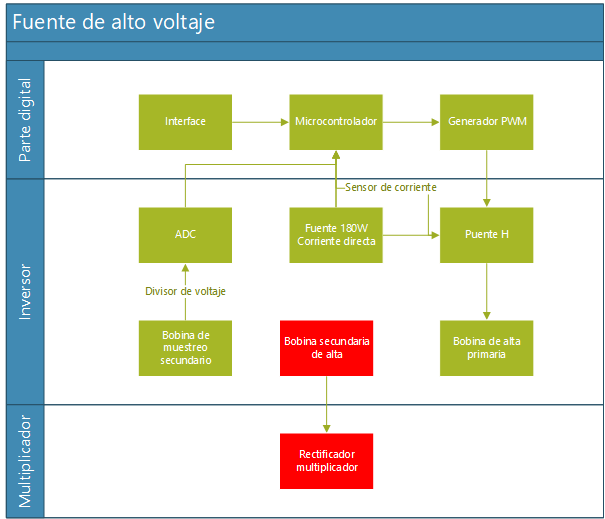
\includegraphics[width=12cm]{Capitulo3/figs/diagrama.png}
\caption{Topología de fuente de alto voltaje}
\end{figure}
\newpage
\subsection{Hardware de interface}
Para el desarrollo de la interface gráfica se a utilizado un microcontrolador ATMEGA2560, implementado por la facilidad de programación y los tiempos cortos para la conclusión de este proyecto, así como también la implementación de una pantalla TFT-LCD ( Pantalla de cristal líquido de transistores de película fina) y comunicación UART como interfaces gráfica al usuario. Se ha utilizado el hardware de dicha placa y ahorrado tiempo de desarrollo. \\


\begin{figure}[H]
\centering
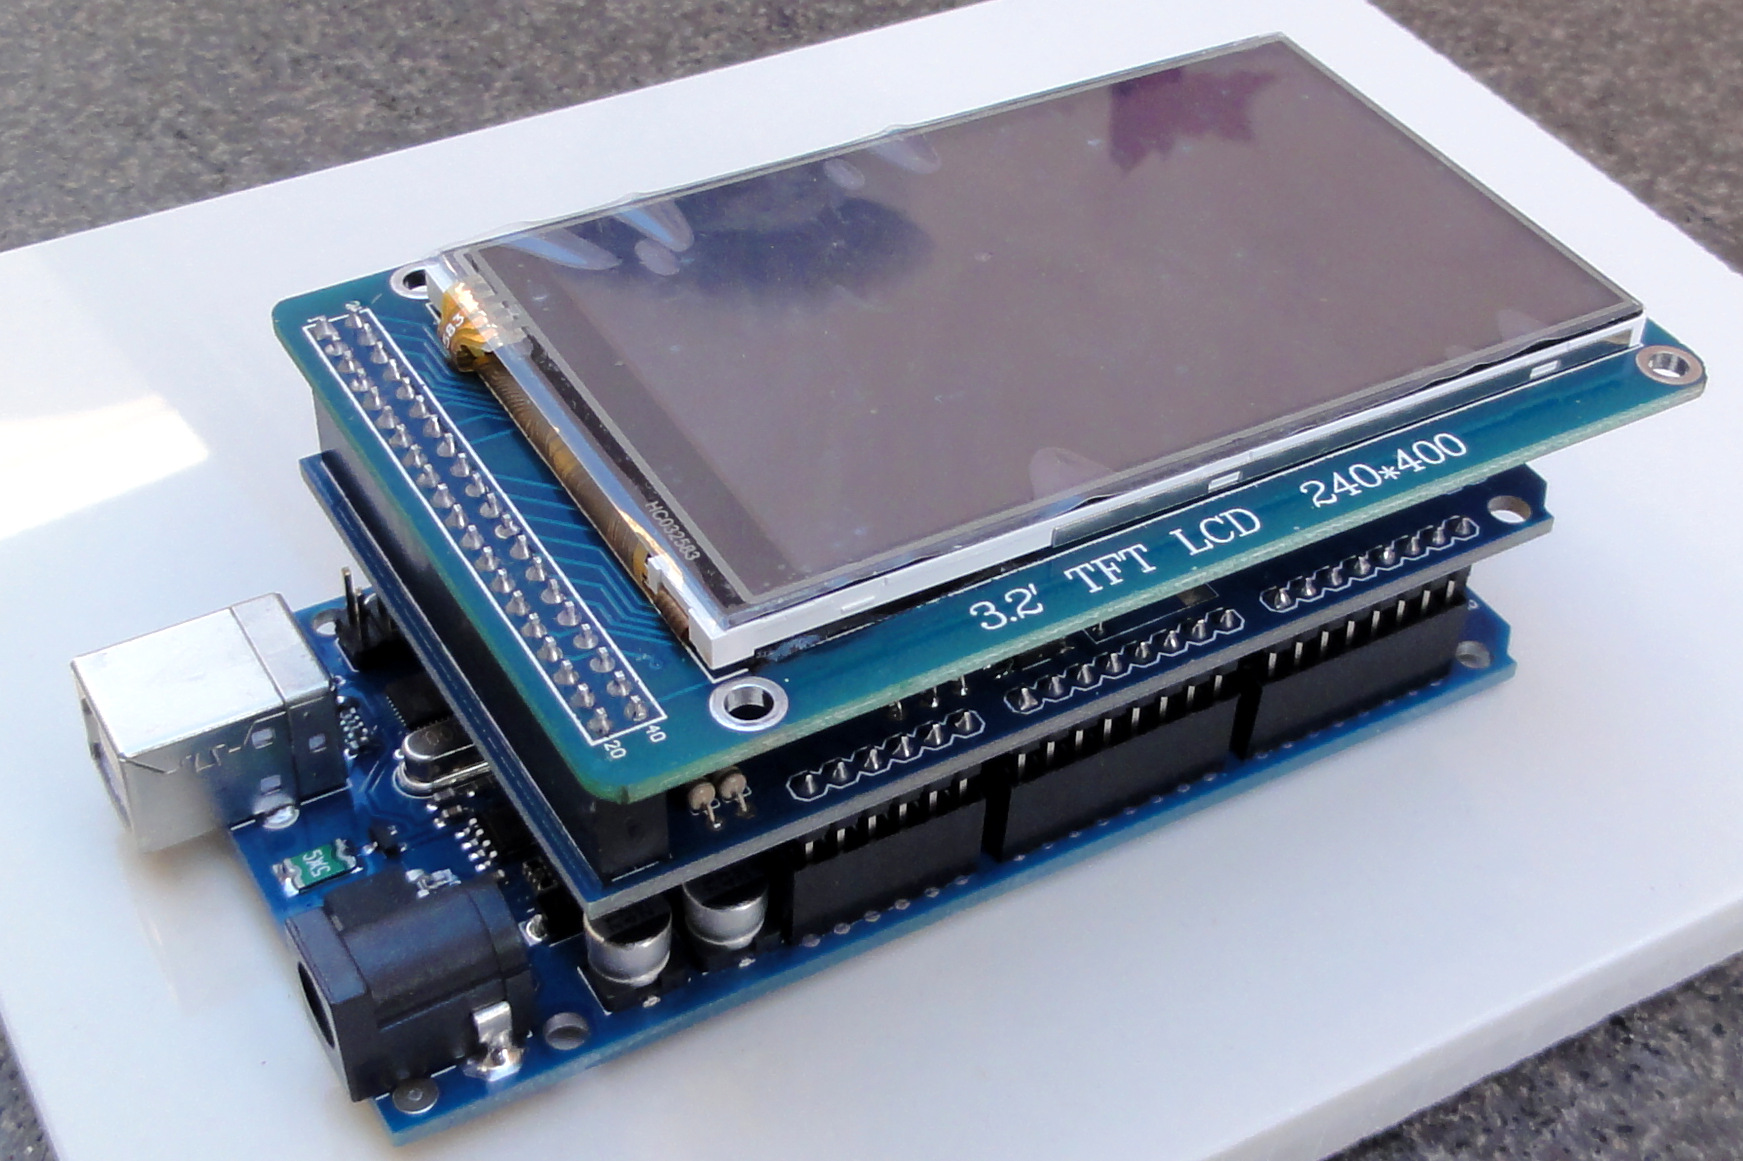
\includegraphics[width=9cm]{Capitulo3/figs/pantalla0.jpg}
\caption{LCD-TFT para interface gráfica}
\end{figure}
\newpage
\subsection{Hardware de fuente de voltaje a 180w}

Esta sección consiste en varias etapas de desarrollo, para ello primero se ha desarrollado una fuente de voltaje de 180W, que es el primer circuito a analizar. Podemos observar en la figura 3.7 el diseño propuesto. El cual esta conformado por el regulador de voltaje LM723 en modalidad fuente de voltaje por modalidad de regulación positiva.\\

Se ha simulado esta fuente de voltaje en el programa LTSPICE como se muestra en la figura 3.8, en este punto se busca el menor rizo posible en nuestra salida final, ya que, en este punto el ruido sera amplificado cientos de veces. Podemos observar en la figura 3.9 que nuestra simulación se acerca bastante a lo buscado, una señal de 12v en corriente directa, teniendo una señal estabilizada en un tiempo de 24ms, suficientemente pequeño para la inicialización de nuestro proyecto. El diseño del PCB se encuentra en la figura 3.10, el cual fue diseñado en el programa EAGLE.\\

\begin{figure}[H]
\centering
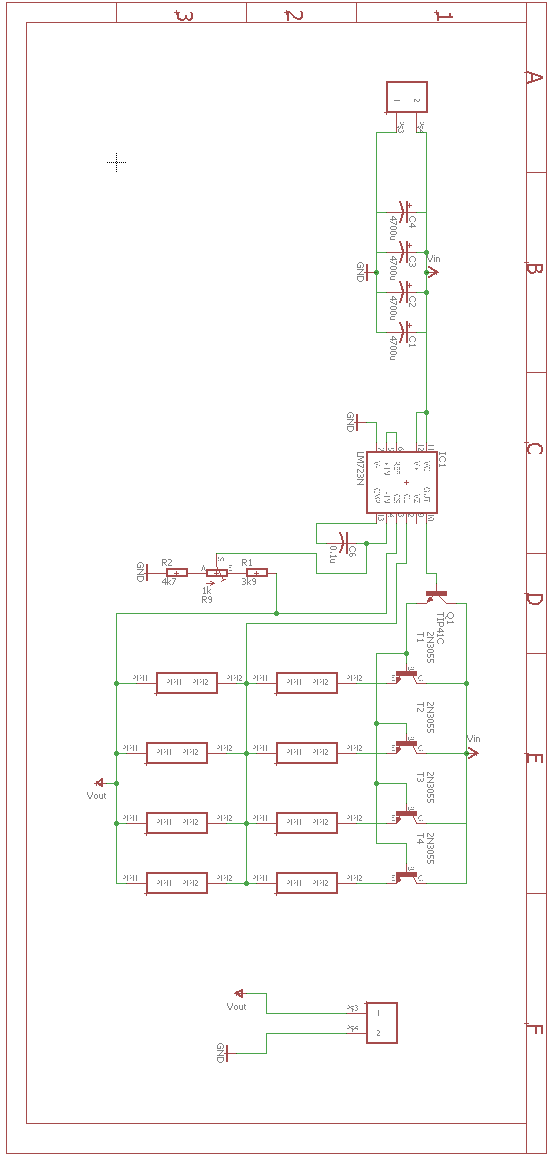
\includegraphics[width=10cm]{Capitulo3/figs/fuente.png}
\caption{Simulación en LTSPICE fuente 180w}
\end{figure}

\begin{figure}[H]
\centering
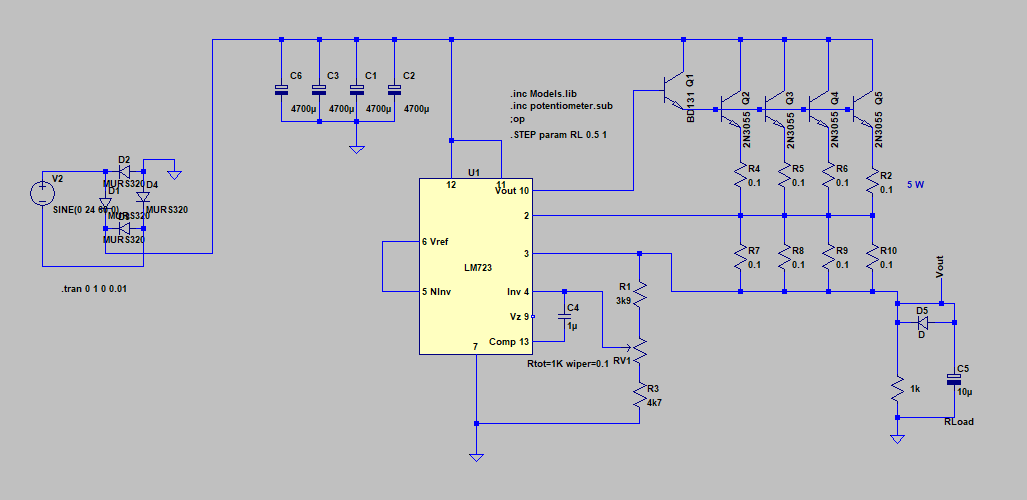
\includegraphics[width=12cm]{Capitulo3/figs/SIMFUENTE.png}
\caption{Simulación en LTSPICE fuente 180w}
\end{figure}




\begin{figure}[H]
\centering
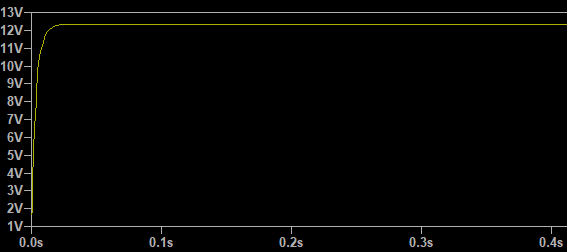
\includegraphics[width=12cm]{Capitulo3/figs/12v.png}
\caption{Simulación fuente regulable en LTSPICE}
\end{figure}

\begin{figure}[H]
\centering
\includegraphics[width=11cm]{Capitulo3/figs/pcb.png}
\caption{Diseño placa de fuente de regulable de 180w}
\end{figure}





\newpage

\subsection{Hardware inversor}

Para el inversor se ha implementado una topología del tipo puente H, ya que es una de las mas utilizadas por los desarrolladores. El integrado BTS7960B \cite{databts} es un mosfet de potencia bastante robusto y con una comunidad de desarrollo bastante grande, es por ello que se ha seleccionado este modelo entre los miles que existen en el mercado. Podemos observar el diagrama implementado en la figura 3.12 \cite{ibt} y partiendo de el se ha utilizado la placa de desarrollo IBT2 (figura 3.11) por cuestión de costos. \\

\begin{figure}[H]
\centering
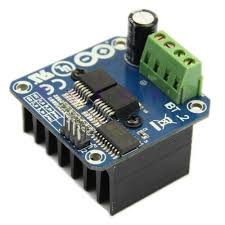
\includegraphics[width=6cm]{Capitulo3/figs/bts.jpg}
\caption{Placa de desarrollo, puente H IBT-2}
\end{figure}

\begin{figure}[H]
\centering
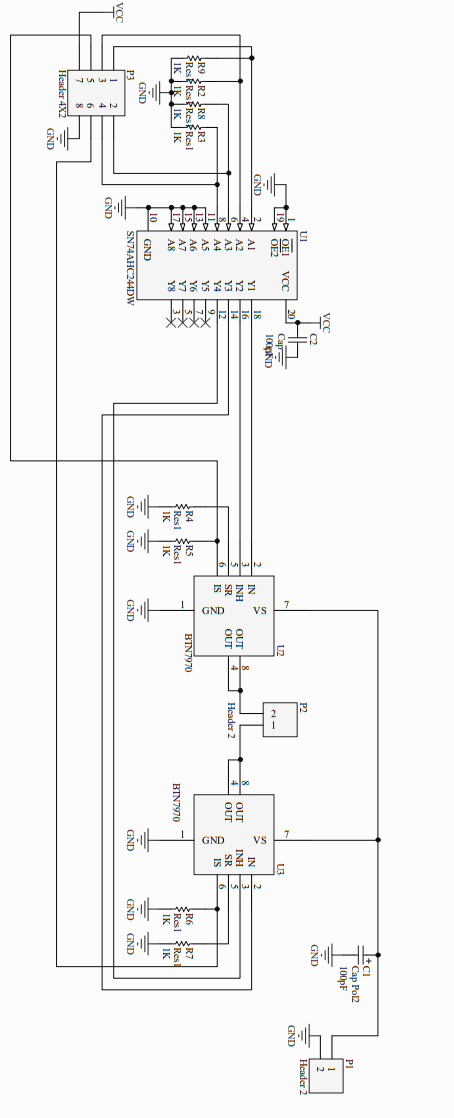
\includegraphics[width=6cm]{Capitulo3/figs/ibt2.png}
\caption{diagrama puente H}
\end{figure}



\newpage


\subsection{Multiplicador de voltaje Cockroft Walton}
Mediante el motor de simulación de LTSPICE se ha realizado el diseño del multiplicador a utilizar. Contando con valores de capacitores de 0.1 $\mu$-Faradios, diodos MUR4100, voltaje de entrada de 1KV y una frecuencia variable de 10KHZ. Podemos observar en la figura 3.9 el diseño planteado, con la finalidad de tener un punto de referencia al momento de realizar el experimento. Se busca tener un rizo menor al 1\% del voltaje de salida y tomaremos la simulación como punto de partida para la construcción del multiplicador. \\

\begin{figure}[H]
\centering
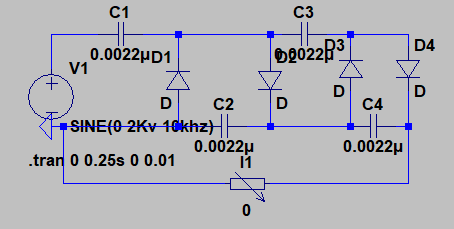
\includegraphics[width=12cm]{Capitulo3/figs/multi.png}
\caption{Multiplicador de voltaje 2 niveles}
\end{figure}

Se han realizado corridas en el simulador con cargas que exigen 1 mA, 10 mA y pruebas sin carga. Podemos observar en la figura 3.14 la salida de CD que se obtiene cuando no tenemos carga alguna, como vemos la salida esta aparentemente libre de rizo y este es el punto de referencia para medir la eficiencia de nuestra fuente. El voltaje en color rojo es la primera etapa de nuestro multiplicador, en color azul tenemos la segunda etapa y en color verde la entrada de corriente alterna. 

\begin{figure}[H]
\centering
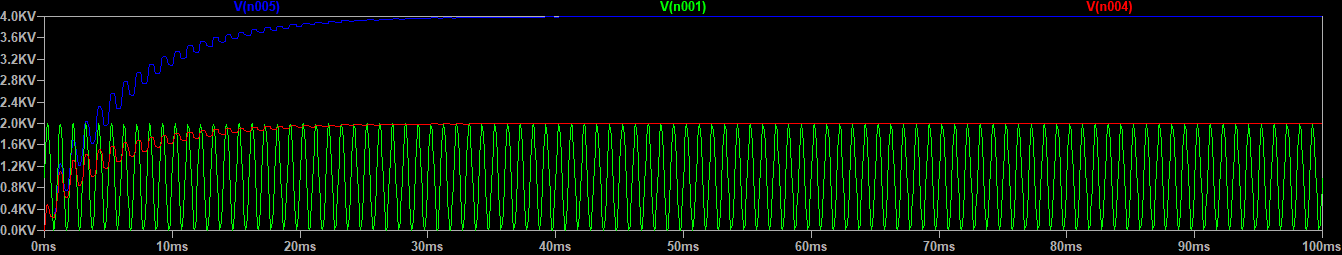
\includegraphics[width=12cm]{Capitulo3/figs/4kv.png}
\caption{Multiplicador de voltaje sin carga}
\end{figure}


Para una carga con una exigencia de 1 mA podemos observar la figura 3.15. Como vemos ahora el rizo y la caída en el voltaje es perceptible a simple vista.


\begin{figure}[H]
\centering
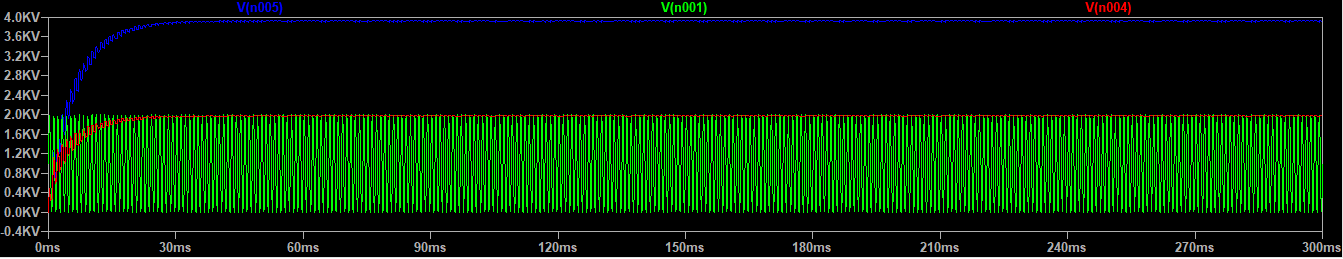
\includegraphics[width=12cm]{Capitulo3/figs/1ma.png}
\caption{Multiplicador de voltaje con 1 mA de carga}
\end{figure}

Para una carga con una exigencia de 10 mA podemos observar la figura 3.16. Tenemos una caída de voltaje bastante significativa y un rizo bastante pronunciado.


\begin{figure}[H]
\centering
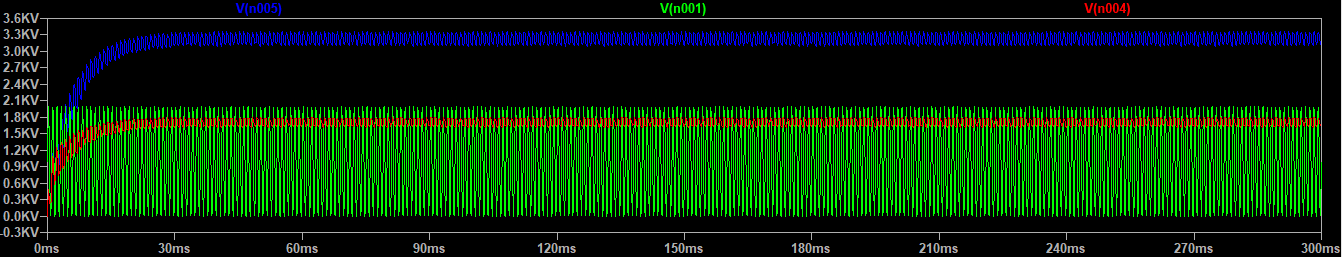
\includegraphics[width=12cm]{Capitulo3/figs/10ma.png}
\caption{Multiplicador de voltaje con 10 mA de carga}
\end{figure}

Tenemos un voltaje $V_{1mA}=3.9KV$, $V_{10mA}=3.2KV$ y $V_{NL}=4KV$ ahora utilizando la ecuación 2.7 podemos calcular la eficiencia de nuestra fuente y utilizar este punto de referencia para la construcción de nuestro proyecto. Para una carga de 1 mA tenemos $VR_{1mA}=2.5\%$ Y para una carga de 10 mA $VR_{10mA}=20\%$ valor límite para nuestro circuito. Caidas de voltaje aceptables para nuestros propósitos.\\

Hasta aquí podemos capturar los siguientes datos importantes, para una carga de 1 mA tenemos una caída de voltaje de 100V y para una carga de 10 mA se tiene una caída de 800V, estos valores son muy grandes, es por ello que se tendrán que ajustar mediante un circuito de retroalimentación. 
\newpage

\section{Firmware}
\subsection{Interface gráfica}
Para el desarrollo de la interface gráfica se ha realizado en el ambiente de programación de Arduino, intentando la utilización de la menor cantidad de librerías de autoría no propia y siguiendo algunas reglas de programación básicas para micro-controladores como lo es la no utilización de los comando delay. Dicho código se divide en varias secciones, para el cual solo se utilizaron las siguientes librerías:

\begin{verbatim}

#include <UTFT.h>
#include <URTouch.h>

\end{verbatim}

En la siguiente figura podemos observar la topología del firmware que se ha desarrollado.\\

\begin{figure}[H]
\centering
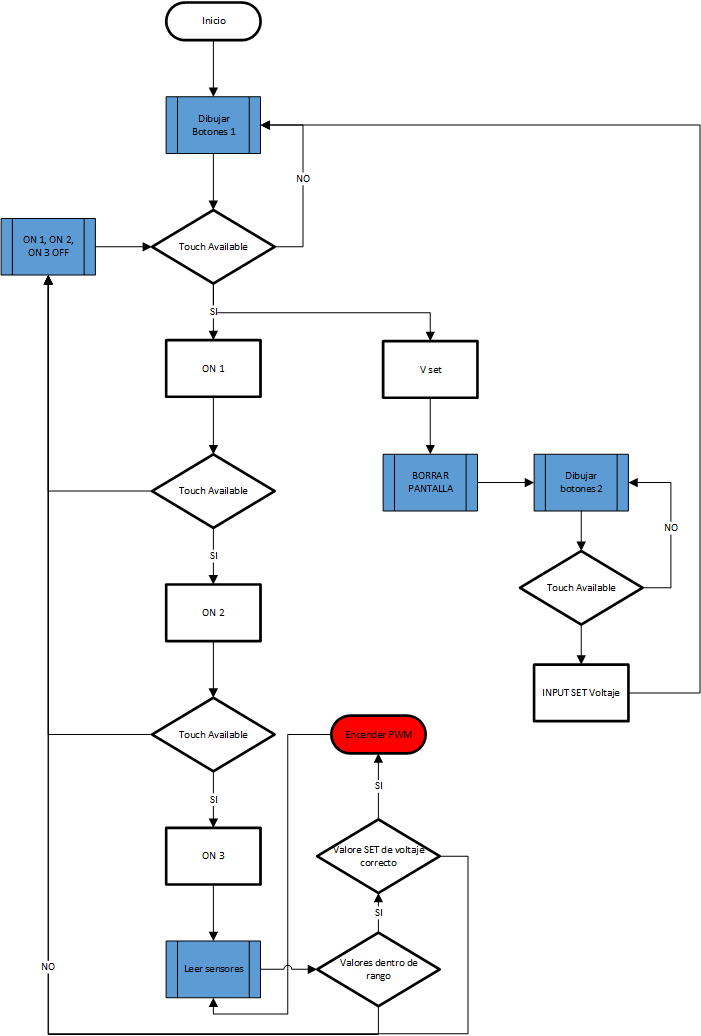
\includegraphics[width=12cm]{Capitulo3/figs/diagramafir.png}
\caption{Multiplicador de voltaje con 10 mA de carga}
\end{figure}


El microcontrolador cuenta con múltiples salidas que permiten una comunicación con el Hardware desarrollado, se han definido las siguientes variables, salidas y entradas del micro controlador.

\begin{verbatim}

void setup(){

  myGLCD.InitLCD();
  myGLCD.clrScr();
  myTouch.InitTouch();
  myTouch.setPrecision(PREC_HI);
  Serial.begin(9600);
  Serial.setTimeout(50);
  }

//Definimos fuentes que utilizaremos
extern uint8_t SmallFont[];
extern uint8_t BigFont[];
extern uint8_t SevenSegNumFont[];

//variables que estaremos utilizando
int x,y,pantalla=1,k,voltaje=1,p=0,p1=0,p2=0,p3=0,vout=0;
char dato[20];

//variables para tomar datos de UART

String str = "";
const char separator = ',';
const int dataLength = 2;
int data[dataLength];
char vin[20];
char current[20];

\end{verbatim}

Como vemos se ha utilizado la función setTimeout, configuración de la comunicación serial, necesaria en el proyecto para mantener una medición de datos sin riesgos a perdida de informacion debido a los subprocesos que se realizan dentro del firmware diseñado. SetTimeout() establece los milisegundos máximos para esperar los datos de transmisión, por defecto es de 1000 milisegundos. Esta función es parte de la clase Stream y es llamada por cualquier clase que hereda de ella (Wire, Serial, etc.). \cite{settime}\\


Todo el código esta dividido en funciones, las cuales llamamos en nuestro LOOP, tratando siempre de cumplir con las siguientes características: no utilización de la función delay, no utilización de ciclos que dependa de alguna condición externa, utilizar el menor código posible para una acción. podemos observar el resultado de nuestro desarrollo en las imagenes 3.18 y 3.19.\\

\begin{figure}[H]
\centering
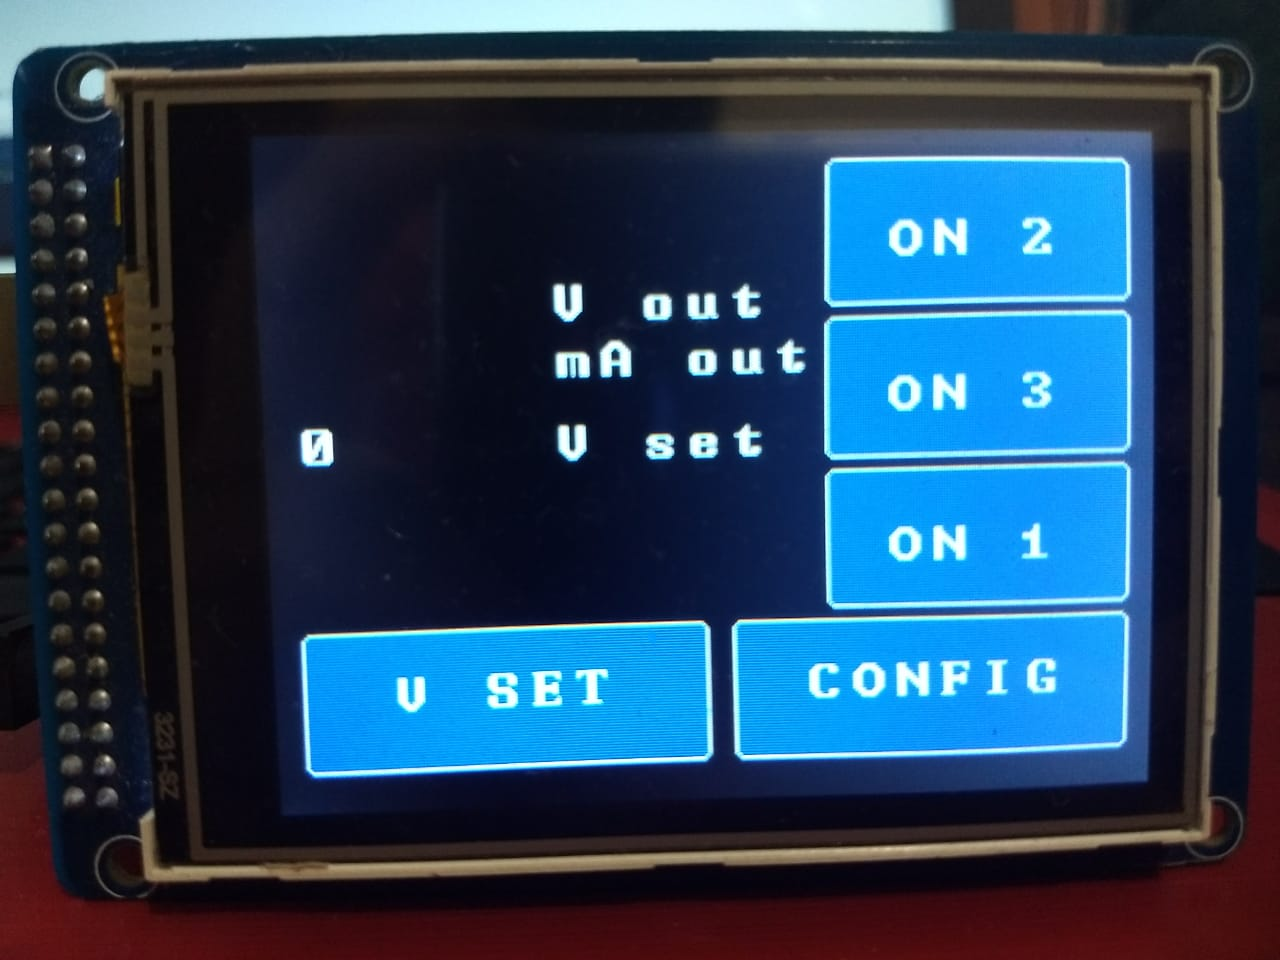
\includegraphics[width=9cm]{Capitulo3/figs/pantalla1.jpg}
\caption{Pantalla 1}
\end{figure}

\begin{figure}[H]
\centering
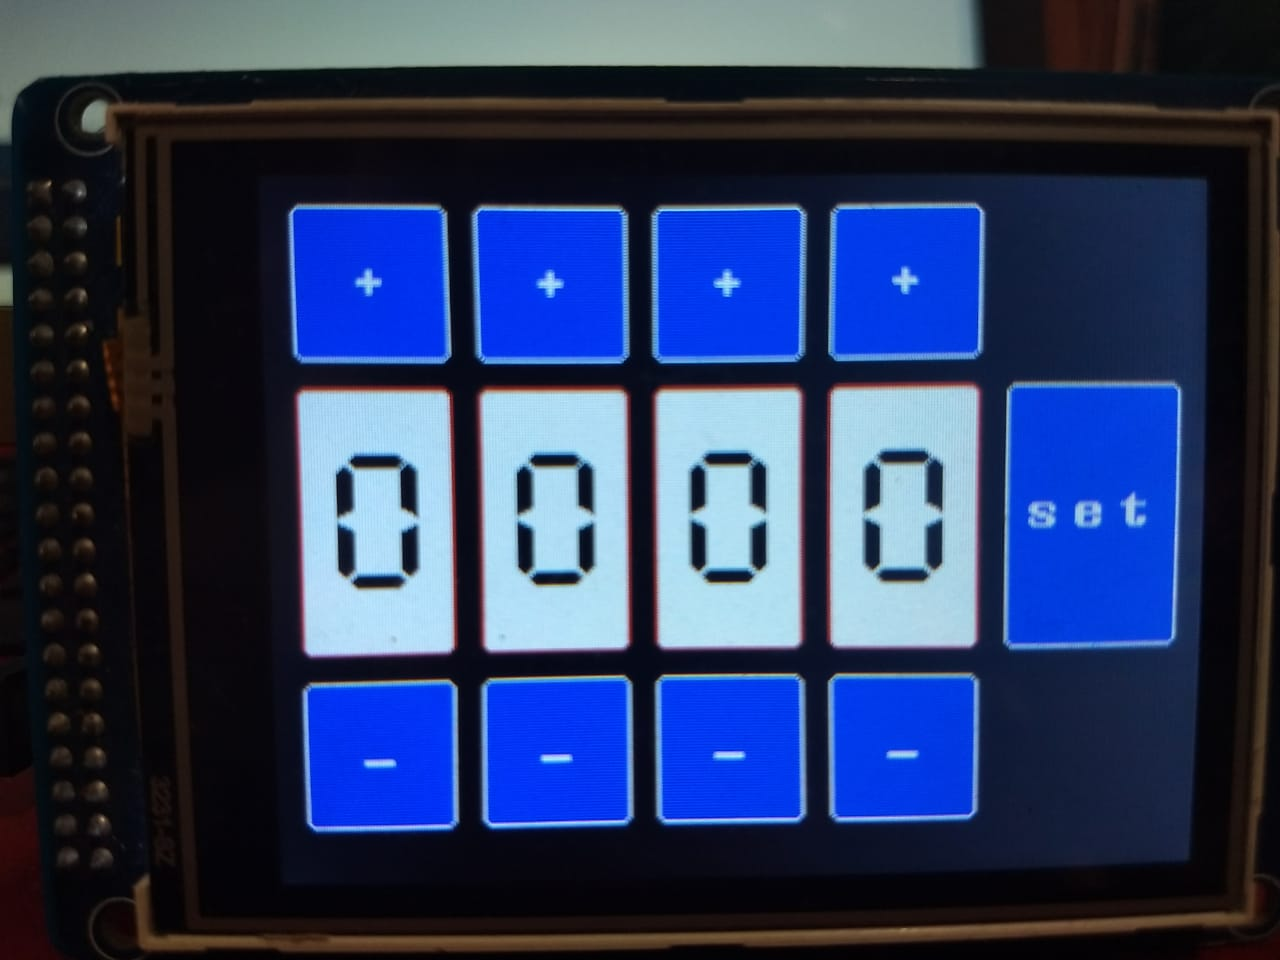
\includegraphics[width=9cm]{Capitulo3/figs/pantalla2.jpg}
\caption{Pantalla 2}
\end{figure}

Una vez que definimos las funciones a utilizar para estas dos primeras pantallas proseguimos a las funciones de cálculos y procesamiento de datos. Para ello hemos creado una función capaz de configurar el voltaje de salida, manteniendo una comunicación UART hacia un micro-controlador. \\

Una segunda función es la encargada de recibir los datos procedentes del segundo micro-controlador, encargado de leer los datos de sensores y preparar el funcionamiento del inversor. \\


Mediante las funciones anteriores podemos mantener una comunicacion INPUT y OUTPUT mediante UART, con el segundo micro-controlador, y mantener un senseo de las variables necesarias para el correcto funcionamiento de la fuente de alto voltaje. Ahora mostramos en cuerpo del programa principal, encargado del control de cada una de las funciones anteriores.

\section{Implementación del Hardware}

Una vez obtenido el diseño de todas las etapas, así como también la programación del firmware se prosigue a la fabricación de los PCB de la fuente de corriente directa a 180W, el acondicionamiento de la parte digital a la etapa de potencia. Se aisló mediante una caja que solo da acceso al usuario a la parte de salidas y entradas como vemos en la imagen 3.20 Evitando así riesgos al usuario. \\


\begin{figure}[H]
\centering
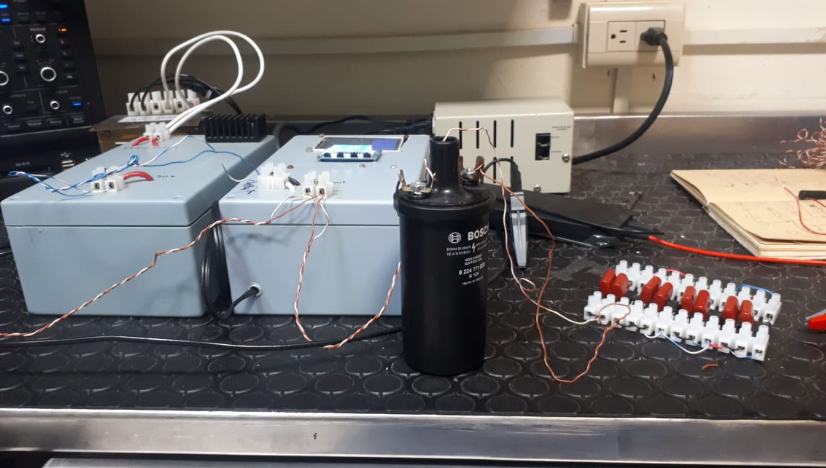
\includegraphics[width=12cm]{Capitulo3/figs/noimagen.png}
\caption{Foto del sistema en general}
\end{figure}

Una vez terminado el Hardware se hicieron pruebas de cada modulo desarrollado, con la finalidad de indicar las condiciones optimas para el sistema en general, haciendo pruebas con diferentes cargas y observando el ruido obtenido de ellos. 

\subsection{Fuente de 180W}

Se ha terminado la maquinación de la fuente de voltaje en el router LPKF y realizado el ensamble. Se tienen 180 W que pueden ser peligrosos si no se tiene el cuidado necesario, es por ello que se ha optado por aislar el circuito y dejar solamente las salidas y entradas necesarias como podemos ver en la imagen 3.21.

\begin{figure}[H]
\centering
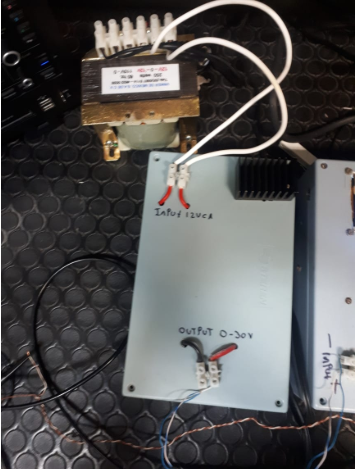
\includegraphics[width=9cm]{Capitulo3/figs/fotofuente.png}
\caption{Multiplicador de voltaje sin carga}
\end{figure}

Se ha optado por hacer pruebas a 12V y cargas de 7.5 OHMS, 15 OHMS y una prueba sin carga, esperando obtener el menor ruido posible. La configuración para el experimento se puede observar en la figura 3.17. Mediante estos resultados se ha creado una gráfica gaussiana para determinar el voltaje RMS en cada experimento. Para ello se implemento el siguiente codigo desarrollado en ''ROOT CERN":\\

 

\begin{verbatim}

#include "Riostream.h"
#include "TH1.h"
#include "TMath.h"
#include "TF1.h"
#include "TLegend.h"
#include "TCanvas.h"
#include <stdio.h>
#include <stdlib.h>
#include <cstdlib>


void clase() {
   ifstream in; ofstream outfile;
   int i,j;
   int z,suma=0;

float n,time;
double x,y,xx,yy;
  TH1 *histo1 = new TH1F("Arrival distribution","", 50, 11.8,12.4);

in.open("C1600v-4M00001.txt"); 

while (1) {

	if (!in.good()) break;
       in >> x;
       
histo1->SetFillColor(4);
		  histo1->Fill(x);				    
	}
	   
 in.close();	  

histo1->Draw();
}
\end{verbatim}

Se han obtenido como resultado las siguientes distribuciones:

\begin{figure}[H]
\centering
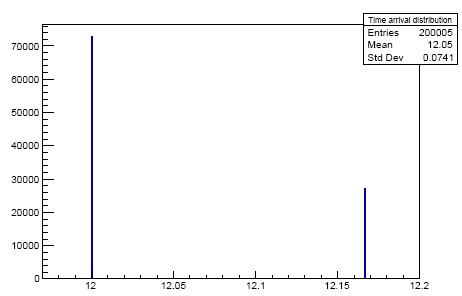
\includegraphics[width=12cm]{Capitulo3/figs/sincarga.png}
\caption{Fuente 12V sin carga con error de 0.076V}
\end{figure}

\begin{figure}[H]
\centering
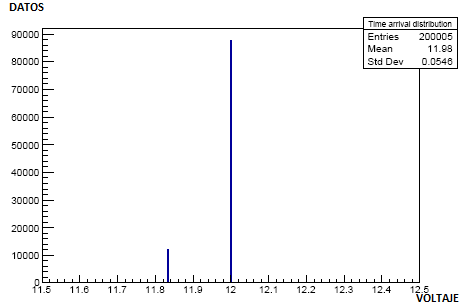
\includegraphics[width=12cm]{Capitulo3/figs/75ohms.png}
\caption{Fuente 12V con carga a 7.5 OHMS con error de 0.076V}
\end{figure}

\begin{figure}[H]
\centering
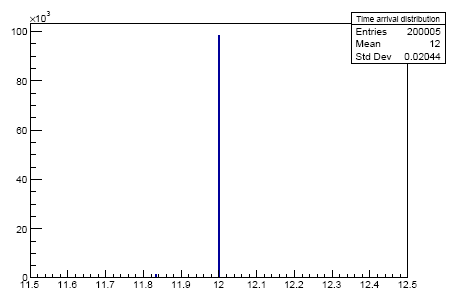
\includegraphics[width=12cm]{Capitulo3/figs/15ohms.png}
\caption{Fuente 12V con carga a 15 OHMS con error de 0.076V}
\end{figure}

Como observamos nuestro RMS se mantiene desde 0.0471v sin carga a 0.0546V con una carga de 7.5 ohms o 90w, con un error asociado a el de 0.076V, ya que nuestro osciloscopio es de 8 bits, obteniendo una regulación de voltaje de $\%VR=0.0627\% $ que significa una eficiencia del 99.93\% cuando la fuente es sometida a una carga resistiva de 90w, eficiencia bastante buena para los experimentos siguientes. \\

Utilizando la ecuación 2.6 obtenemos los siguientes resultados en rizo:\\

 
 Para $12V$ sin carga: $$r=\frac{0.0741}{12.05V}X100=0.61 \% $$ 
 
 Para $12V$ con carga de 7.5 ohms: $$r=\frac{0.0546V}{11.98V}X100=0.45 \% $$ 
 
 Para $12V$  con carga de 15 ohms: $$r=\frac{0.02044V}{12V}X100=0.170 \% $$



\subsection{Inversor de voltaje}

Este modulo ha sido aislado de la misma manera que se aisló la fuente de 180W (Fig. 3.21), debido a los riesgos que conlleva al usuario si no se tiene el cuidado pertinente. Ahora, utilizando la fuente de 180W y corriente directa se alimenta nuestro inversor. Nuestro inversor tiene dos variables que pueden ajustarse de manera manual o automática; la frecuencia y el ciclo de trabajo. Mediante estas variables de voltaje, incidentes en nuestro primario de la bobina de alto voltaje, podemos variar la salida de alto voltaje y tener un ajuste fino de nos cuantos volts por paso.\\

Tener cargas inductivas muchas veces puede volver mas complicado la implementación de nuestros circuitos, agregando armónicos y corrientes que pueden comportarse de manera no esperada. Podemos observar en la figura 3.26 la salida de nuestro inversor agregando una carga inductiva, un ciclo de trabajo del 5\% y una frecuencia de 5 KHz. Podemos observar que nuestra señal AC mantiene su forma.

\begin{figure}[H]
\centering
\includegraphics[width=9cm]{Capitulo3/figs/inversor.png}
\caption{Implementacion experimento inversor.}
\end{figure}

\begin{figure}[H]
\centering
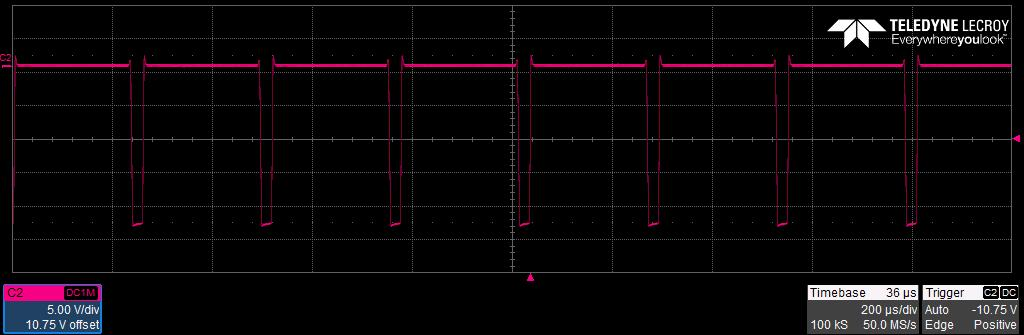
\includegraphics[width=12cm]{Capitulo3/figs/pwm1.jpg}
\caption{Implementación inversor salida con carga inductiva.}
\end{figure}



\subsection{Multiplicador de voltaje}

Existen aspectos claves para este apartado que definirán la calidad de nuestra salida, es por ello que se han realizado pruebas variando algunos aspectos como lo son la frecuencia y el ciclo de trabajo incidente en la bobina primaria del transformador de alto voltaje. Podemos observar un circuito provisional desarrollado (figura 3.27) y mediante mediciones sin carga se han obtenido principalmente dos valores, el voltaje medio y el voltaje RMS, para obtener el rizo sobre dicha señal.



\begin{figure}[H]
\centering
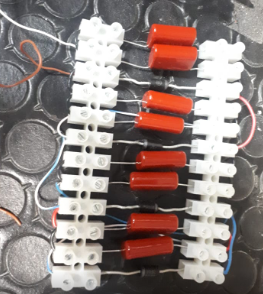
\includegraphics[width=9cm]{Capitulo3/figs/fotomulti.png}
\caption{Implementación inversor}
\end{figure}

\begin{figure}[H]
\centering
\includegraphics[width=9cm]{Capitulo3/figs/93V.jpg}
\caption{Medición sin carga a 93v con un error de 0.36V}
\end{figure}

\begin{figure}[H]
\centering
\includegraphics[width=9cm]{Capitulo3/figs/200V.jpg}
\caption{Medición sin carga a 200V con un error de 0.78V}
\end{figure}

\begin{figure}[H]
\centering
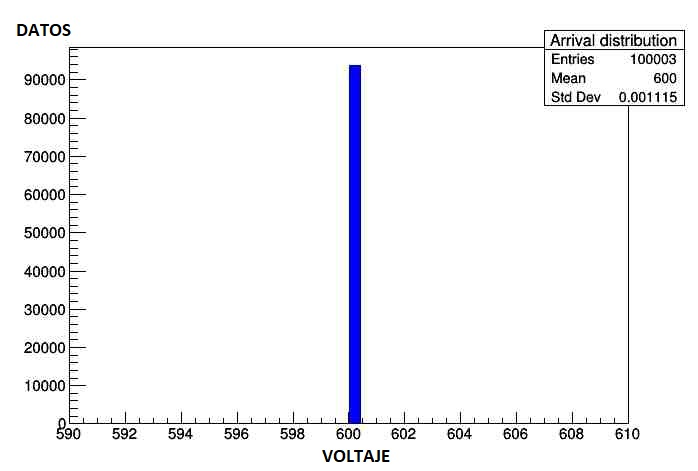
\includegraphics[width=9cm]{Capitulo3/figs/600v.jpg}
\caption{Medición sin carga a 600V con un error de 2.34V}
\end{figure}

\begin{figure}[H]
\centering
\includegraphics[width=9cm]{Capitulo3/figs/986V.jpg}
\caption{Medición sin carga a 986V con un error de 3.85V}
\end{figure}

A partir de estas mediciones podemos calcular el rizo que tiene nuestra medición utilizando la ecuación 2.4 como podemos observar en las figuras 3.28, 3.29, 3.30 y 3.31  respectivamente. \\

Para la medición a $93V$ tenemos:

 $$r=\frac{4.157V}{94.79V}X100=4.3 \% $$ 
 
 Para $200V$: $$r=\frac{0.00027V}{200V}X100=135\mu \% $$ 
 
 Para $600v:$  $$r=\frac{0.001115V}{600V}X100=185\mu \% $$ 
 
 Para $1000V$  $$r=\frac{0.002435V}{986V}X100=246.7\mu \% $$

El segundo experimento que se realizo fue agregar una carga de $4M\Omega$ para obtener la eficiencia de la misma, valor calculado con la ecuación 2.7. \\

Para $93V$ $V_{NL}=186V$ y $V_{FL}=100V$: $$\%VR=\frac{V_{NL}-V_{FL}}{V_{FL}}=\frac{186V-100V}{186V}X100= 86 \% $$

Para $300V$ $V_{NL}=577V$ y $V_{FL}=300V$ : $$\%VR=\frac{V_{NL}-V_{FL}}{V_{FL}}X100=\frac{577V-300V}{300V}X100= 92\% $$

Los valores importantes para definir la eficiencia de una fuente son el rizo que existe sobre el voltaje de corriente directa y la caída de voltaje con una carga respectiva. En nuestro caso se tienen caídas de voltaje de hasta el 92\%, debido a que no se cuenta con una retroalimentación necesaria. 
